\section{Часть I: Протоколы и монотонные модели}

\begin{frame}
    \centering
    \usebeamerfont{title}\insertsectionhead

    \vspace{0.3cm}
    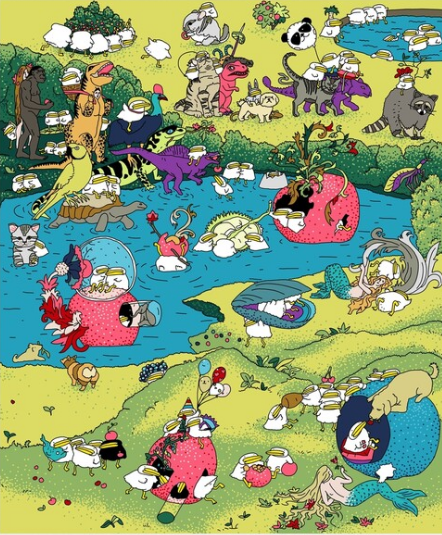
\includegraphics[scale = 0.3]{pics/utia-garden.png}
\end{frame}

\begin{frame}{Монотонные модели}

    \begin{minipage}{0.33\linewidth}
        \centering
        Формулы
        \vspace{0.2cm}
        
        \begin{tikzpicture}[>=latex]
    \node[circle, minimum size = 0.5cm, inner sep = 0pt, draw, fill = LEIorange!5] (a) at (5, 2)
        {$x$};
    \node[circle, minimum size = 0.5cm, inner sep = 0pt, draw, fill = LEIorange!5] (b) at (3.5, 2)
        {$y$};
    \node[circle, minimum size = 0.5cm, inner sep = 0pt, draw, fill = LEIorange!5] (c) at (4.5, 1)
        {$\lor$};
    \node[circle, minimum size = 0.5cm, inner sep = 0pt, draw, fill = LEIorange!5] (d) at (2.7, 1)
        {$z$};
    \node[circle, minimum size = 0.5cm, inner sep = 0pt, draw, fill = LEIorange!5] (e) at (3.8, 0.3)
        {$\land$};
    \node[circle, minimum size = 0.5cm, inner sep = 0pt, draw, fill = LEIorange!5] (f) at (5.2, 0.6)
        {$y$};
    \node[circle, minimum size = 0.5cm, inner sep = 0pt, draw, fill = LEIorange!5] (g) at (4, -0.5)
        {$\lor$};

    \draw[->] (a) -- (c);
    \draw[->] (b) -- (c);
    \draw[->] (c) -- (e);
    \draw[->] (d) -- (e);
    \draw[->] (e) -- (g);
    \draw[->] (f) -- (g);
    \draw[->] (g) -- ++(0, -0.5);
\end{tikzpicture}
    \end{minipage}
    \begin{minipage}{0.33\linewidth}
        \centering
        Схемы
        \vspace{0.2cm}
        
        \begin{tikzpicture}[>=latex]
    \node[circle, minimum size = 0.5cm, inner sep = 0pt, draw, fill = LEIorange!5] (a) at (5, 2)
        {$x$};
    \node[circle, minimum size = 0.5cm, inner sep = 0pt, draw, fill = LEIorange!5] (b) at (3.5, 2)
        {$y$};
    \node[circle, minimum size = 0.5cm, inner sep = 0pt, draw, fill = LEIorange!5] (c) at (4.5, 1)
        {$\lor$};
    \node[circle, minimum size = 0.5cm, inner sep = 0pt, draw, fill = LEIorange!5] (d) at (2.7, 1)
        {$z$};
    \node[circle, minimum size = 0.5cm, inner sep = 0pt, draw, fill = LEIorange!5] (e) at (3.8, 0.3)
        {$\land$};
    %\node[circle, minimum size = 0.5cm, inner sep = 0pt, draw, fill = LEIorange!5] (f) at (5.2, 0.6)
     %   {$y$};
    \node[circle, minimum size = 0.5cm, inner sep = 0pt, draw, fill = LEIorange!5] (g) at (4, -0.5)
        {$\lor$};

    \draw[->] (a) -- (c);
    \draw[->] (b) -- (c);
    \draw[->] (c) -- (e);
    \draw[->] (d) -- (e);
    \draw[->] (e) -- (g);
    \draw[->] (c) -- (g);
    \draw[->] (g) -- ++(0, -0.5);
\end{tikzpicture}
    \end{minipage}
    \begin{minipage}{0.32\linewidth}
        \centering
        Еще схемы
        \vspace{0.2cm}
        
        \begin{tikzpicture}[>=latex]
    \node[circle, minimum size = 0.5cm, inner sep = 0pt, draw, fill = LEIorange!5] (a) at (5, 2)
        {$x$};
    \node[circle, minimum size = 0.5cm, inner sep = 0pt, draw, fill = LEIorange!5] (b) at (3.5, 2)
        {$y$};
    \node[circle, minimum size = 0.5cm, inner sep = 0pt, draw, fill = LEIorange!5] (c) at (4.5, 1)
        {$+$};
    \node[circle, minimum size = 0.5cm, inner sep = 0pt, draw, fill = LEIorange!5] (d) at (2.7, 1)
        {$3$};
    \node[circle, minimum size = 0.5cm, inner sep = 0pt, draw, fill = LEIorange!5] (e) at (3.8, 0.3)
        {$*$};
    %\node[circle, minimum size = 0.5cm, inner sep = 0pt, draw, fill = LEIorange!5] (f) at (5.2, 0.6)
     %   {$y$};
    \node[circle, minimum size = 0.5cm, inner sep = 0pt, draw, fill = LEIorange!5] (g) at (4, -0.5)
        {\scriptsize $\mathrm{exp}$};

    \draw[->] (a) -- (c);
    \draw[->] (b) -- (c);
    \draw[->] (c) -- (e);
    \draw[->] (d) -- (e);
    \draw[->] (e) -- (g);
    \draw[->] (c) -- (g);
    \draw[->] (g) -- ++(0, -0.5);
\end{tikzpicture}
    \end{minipage}

    \pause
    Зачем нужны нижние оценки?
    \begin{itemize}
        \item Ведь получается!
            \pause
        \item Контроль погрешности.
            \pause
        \item Сильные монотонные оценки $\Rightarrow$ оценки на все схемы.
            \pause
        \item Задача о разделении секрета.
    \end{itemize}
\end{frame}


\begin{frame}{Ранние результаты}
    \pause
    Оценки на схемы:
    \begin{itemize}
        \item{} [Разборов 85] Задача о клике. $n^{\omega(1)}$.
        \item{} [Alon, Boppana 87] Задача о клике. $2^{n^{\varepsilon}}$.
        \item{} [Tardos 87] Задачи <<типа>> клики. $\mathbf{mon}\P$ vs $\P$.
        \item{} [Pudlak 97] Задача о клике. Вещественные схемы. $2^{n^{\varepsilon}}$.
        \item{} [Harnik, Raz 03] Спец. функция. $2^{\sqrt[3]{n}}$.
    \end{itemize}

    \vspace{0.5cm}
    \pause
    Оценки на формулы:
    \begin{itemize}
        \item{} [Karchmer, Wigderson 90] Задача о достижимости в графе. $n^{\log n}$.
        \item{} [Raz, McKenzie 99] Большой класс спец. функций. $2^{\sqrt{n}}$.
    \end{itemize}
\end{frame}



\begin{frame}{Коммуникационные протоколы. $f\colon U \times V \to T$}
    \begin{center}
    	\onslide<1->{
    \tikzstyle{op1} = [opacity = 0]
    \tikzstyle{op2} = [opacity = 0]
    \tikzstyle{op3} = [opacity = 0]
    \tikzstyle{op4} = [opacity = 0]
}
\only<2->{\tikzstyle{op2} = [opacity = 1]}
\only<3->{\tikzstyle{op3} = [opacity = 1]}
\only<4->{\tikzstyle{op4} = [opacity = 1]}

\begin{tikzpicture}[black]
    \node[police, female, minimum size = 1.5cm] (alice) at (0, 0) {};
    \node[jester, mirrored, minimum size = 1.5cm] (bob) at (7, 0) {};
    \node[above = 0.3 of alice] {$x \in U$};
    \node[above = 0.3 of bob] {$y \in V$};

    \path (alice.east) -- (bob.west) node[midway, above = 2.3] {\Large $f(x, y) = ?$};
    \draw[op2, ->, thick] ($(alice.east) + (0.3, 1)$) -- ($(bob.west) + (-0.3, 1)$) node[midway, above] {$r_1 = a(x)$};
    \draw[op3, <-, thick] ($(alice.east) + (0.3, 0.2)$) -- ($(bob.west) + (-0.3, 0.2)$) node[midway, above] {$r_2 = b(y,
        r_1)$};
    \draw[op4, ->, thick] ($(alice.east) + (0.3, -0.2)$) -- ($(bob.west) + (-0.3, -0.2)$);
    \draw[op4, ->, thick] ($(alice.east) + (0.3, -0.6)$) -- ($(bob.west) + (-0.3, -0.6)$) node[midway, below] {$\vdots$};
\end{tikzpicture}    
    \end{center}

    \pause
    \pause
    \pause
	\pause

    \begin{itemize}
        \item Глубина~--- число раундов в худшем случае.
        \item $\DCC(f) = \min\limits_{P \in \mathcal{P}} \mathrm{depth}(P)$, где $\mathcal{P}$ протоколы
            для $f$.
    \end{itemize}
\end{frame}

\begin{frame}{Протоколы и деревья}

    Алиса получает $u \in U$, Боб $v \in V$. Протокол~--- это дерево:

    \begin{columns}[t]
		\begin{column}{0.7\textwidth}
            \begin{itemize}
                \item<2-> вершины помечены игроками;
    		    \item<8-> листья ответами.
	        \end{itemize}

    		\onslide<9->{
                Размер протокола~--- размер дерева. $\mathrm{Size}(f) = \min\limits_{P \in \mathcal{P}}
                \mathrm{Size}(P)$.
            }
            \onslide<10->{
                \begin{lemma}
                    $\DCC(f) = \Omega(\log(\mathrm{Size}(f)))$.
                \end{lemma}
            }
        \end{column}
        
		\begin{column}{0.25\textwidth}
            \tikzstyle{inner} = [thin, circle, minimum size = 0.3cm, draw, inner sep = 0.1pt, black]
\tikzstyle{inner_g} = [thin, circle, minimum size = 0.3cm, draw, inner sep = 0.1pt, black, fill = green]
\tikzstyle{inner_r} = [thin, circle, minimum size = 0.3cm, draw, inner sep = 0.1pt, black, fill = red]
\tikzstyle{inner_b} = [thin, circle, minimum size = 0.3cm, draw, inner sep = 0.1pt, black, fill = blue!50!white]
\tikzstyle{ed} = [thick, ->, draw, black]

    
\begin{tikzpicture}
    \only<-3, 5->{
        \node[inner] (a) at (0, 0) {\scriptsize $a$};
	}
    \only<4>{
        \node[inner_g] (a) at (0, 0) {\scriptsize $a$};
    }

    \only<-4, 6->{
        \node[inner] (b) at (-0.9, -1.2) {\scriptsize $b$};
	}
    \only<5>{
        \node[inner_g] (b) at (-0.9, -1.2) {\scriptsize $b$};
    }

    \node[inner] (c) at (0.9, -1.2) {\scriptsize $a$};
    \node[inner, label = below:$t_1$] (d) at (-1.5, -2.4) {};

    \only<-5, 7->{
        \node[inner] (e) at (-0.3, -2.4) {\scriptsize $b$};
	}
    \only<6>{
        \node[inner_g] (e) at (-0.3, -2.4) {\scriptsize $b$};
    }

    \node[inner] (e2) at (0.3, -2.4) {\scriptsize $b$};
    \node[inner, label = below:$t_4$] (f) at (1.5, -2.4) {};

    \only<-6, 9->{
        \node[inner, label = below:$t_2$] (g) at (-1.5, -4.3) {};
	}
    \only<7-8>{
        \node[inner_g, label = below:$t_2$] (g) at (-1.5, -4.3) {};
    }
    
    \node[inner, label = below:$t_3$] (h) at (-0.25, -4.3) {};
	\node[inner, label = below:$t_3$] (g2) at (1.5, -4.3) {};
    \node[inner, label = below:$t_2$] (h2) at (0.25, -4.3) {};
    
    \path (a) edge[ed] (b);
    \path (a) edge[ed] (c);
    \path (b) edge[ed] (d);
    \path (b) edge[ed] (e);
    \path (c) edge[ed] (e2);
    \path (c) edge[ed] (f);
    \path (e) edge[ed] (g);
    \path (e) edge[ed] (h);
    \path (e2) edge[ed] (g2);
    \path (e2) edge[ed] (h2);
\end{tikzpicture}

		\end{column}
	\end{columns}

\end{frame}

\begin{frame}{Отношение $\KW$ [Karchmer, Wigderson 90]}
    Пусть $U, V \subseteq \{0, 1\}^{n}$ и $U \cap V = \emptyset$.

    \vspace{0.1cm}
    $\KW$:
    \begin{itemize}
        \item Алиса получает $u \in U$, Боб $v \in V$;
        \item задача найти такой $i$, что $u_i \neq v_i$.
    \end{itemize}
    \pause
    Монотонная версия $\KWm$:
    \begin{itemize}
        \item задача найти такой $i$, что $u_i = 1 \land v_i = 0$.
    \end{itemize}

    \pause

    \begin{theorem}[Karchmer, Wigderson 90]
        \alert{Монотонная} формула для $f$ размера $S$ $\Leftrightarrow$ коммуникационный протокол для
        \alert{$\KWm$} $\KW$, где $U \coloneqq f^{-1}(1), V \coloneqq f^{-1}(0)$.
    \end{theorem}
\end{frame}


\begin{frame}{$\KW^m$~--- <<полное отношение>>}

    \begin{itemize}
        \item $\mathcal{S} \subseteq U \times V \times \mathcal{O}$;
        \item определим $F_{\mathcal{S}}\colon \{0, 1\}^m \to \{0, 1\}$ так, чтобы
            $\DCC(\KWm[F_{\mathcal{S}}]) = \DCC(S)$.
    \end{itemize}

    \pause

    \vspace{-0.2cm}
    \begin{center}
        \tikzstyle{ops} = [alt=<{#1}>{opacity = 1}{opacity = 0}]

\begin{tikzpicture}
    \draw[thick, rounded corners = 2pt] (0, 0) rectangle (4, 3);
    \node at (-0.3, 1.5) {$U$};
    \node at (5, 1.5) {};
    \node at (2, 3.3) {$V$};

    \draw[red!30, fill = red!10, rounded corners = 3pt] (0.3, 0.1) rectangle (1, 2.9)
        node[midway, red!80] {$1\colon o_i$};
    \draw[green!50!black, fill = green!30, rounded corners = 3pt, opacity = 0.5] (0.5, 0.4) rectangle
        (3.5, 0.9) node[midway, green!20!black] {$2\colon o_j$};
    \draw[blue!50!black, fill = blue!30, rounded corners = 3pt, opacity = 0.5] (0.7, 2) rectangle
        (3.4, 2.85) node[midway, blue!20!black] {$3\colon o_k$};
    \draw[ops = 3, very thick, red] (-1, 0.5) -- (5, 0.5);
    \draw[ops = 4, very thick, red] (3, -0.5) -- (3, 3.5);
\end{tikzpicture}
    \end{center}

    \pause
    $F_{\mathcal{S}}(1, 1, 0, \dots) \coloneqq 1$\pause, ~~~$F_{\mathcal{S}}(1, 0, 0, \dots) \coloneqq 0$

    \pause
    \begin{lemma}
        $F_{\mathcal{S}}$ может быть дополнена до монотонной так, что $\DCC(\KWm[F_{\mathcal{S}}]) =
        \DCC(S)$.
    \end{lemma}

    \pause
    \putpos{250}{110}{
\includegraphics[scale = 0.1]{pics/utia-think.png}}

\end{frame}